\documentclass[11pt]{article}
\usepackage[letterpaper,margin=1in]{geometry}
\usepackage{amsmath,amssymb}
\usepackage{booktabs}
\usepackage{graphicx}
\usepackage{setspace}
\usepackage{xurl} % allow line breaks in long URLs
\usepackage[hidelinks]{hyperref}
\usepackage{xcolor}
\usepackage{titlesec}
\usepackage{caption}
\usepackage{longtable}
\usepackage{array}
\usepackage{float}
\usepackage[verbose=silent]{microtype} % better justification; helps avoid overfull boxes

\setlength{\emergencystretch}{2em} % relax line breaking to avoid overfull \hbox warnings

\titleformat*{\section}{\large\bfseries}
\titleformat*{\subsection}{\normalsize\bfseries}

\renewcommand{\thesection}{S\arabic{section}}
\renewcommand{\thesubsection}{S\arabic{section}.\arabic{subsection}}
\renewcommand{\thetable}{S\arabic{table}}
\renewcommand{\thefigure}{S\arabic{figure}}
\renewcommand{\theequation}{S\arabic{equation}}

\title{\textbf{Supplementary Material}\\[0.4em]
\large Calibration-to-Deployment Mismatch in HIV Prevention Trials: How Structural Censoring Biases Counterfactual Incidence Estimates}

\author{A.C. Demidont, DO, AAHIVS\\ Nyx Dynamics LLC, Philadelphia, PA 19107}
\date{May 20, 2026}\begin{document}
\maketitle
\onehalfspacing

\tableofcontents
\vspace{1em}
\hrule
\vspace{1em}
\section{Extended derivations}

\subsection{Exponential approximation of \texorpdfstring{$P_R(t)$}{PR(t)} for the Sedia LAg-EIA}

The closed-form correction $\Omega^* \approx \Omega/(1+\gamma\tau)$ used throughout the main letter (Eq.~3) relies on an exponential approximation of the probability of testing recent as a function of age-of-infection $t$:
\begin{equation}
P_R(t) \;\approx\; P_0 \exp(-t/\tau) \label{eq:PR_exp}
\end{equation}
with $\tau \approx 173$ days for the Sedia LAg-EIA at the conventional recency cutoff (optical density normalized, ODn $<$ 1.5). Under this parameterization, the nominal MDRI evaluates to
\begin{equation}
\Omega = \int_0^T P_R(t)\,dt = P_0 \tau (1 - e^{-T/\tau}) \label{eq:Omega_full}
\end{equation}
and the effective MDRI under constant structural hazard $\gamma$ evaluates to
\begin{equation}
\Omega^*(\gamma) = P_0 \int_0^T \exp(-t/\tau) \exp(-\gamma t)\,dt
= \frac{P_0\tau}{1 + \gamma\tau}\left(1 - e^{-T(1/\tau + \gamma)}\right) \label{eq:Omega_star_full}
\end{equation}
For $T \gg \tau$ (the standard choice $T = 730$ days with $\tau = 173$ days gives $T/\tau \approx 4.2$), both exponential terms approach their asymptotic values and the ratio simplifies to
\begin{equation}
\frac{\Omega^*(\gamma)}{\Omega} \approx \frac{1}{1 + \gamma\tau} \label{eq:Omega_star_closed}
\end{equation}
The approximation is exact in the asymptotic limit $T/\tau \to \infty$ under the exponential $P_R(t)$ basis. Two qualifications attach to its use as an approximation to the true LAg-EIA response.

First, at $T/\tau = 4.2$, the omitted terms in Eqs.~\ref{eq:Omega_full}--\ref{eq:Omega_star_full} contribute approximately $1.5\%$. This is a small under-estimate of the true deflation under the exponential basis itself.

Second, the published Sedia LAg-EIA recency curve is not strictly exponential. It exhibits a delayed onset (near-zero $P_R$ for $t < 30$ days during the eclipse-to-Fiebig-II window) and a longer right tail than strict exponential decay. Calibration against the Sedia-reported empirical $P_R(t)$ curve produces $\Omega^*$ values approximately 2--4\% smaller than the closed-form approximation for a given $\gamma$ in the empirical AIDSVu range. The bias magnitudes reported in the main letter therefore under-estimate the magnitudes that would obtain under exact $P_R(t)$, in the conservative direction.

A separate basis-projection question concerns the screening-side observation factor $\rho_{\mathrm{screen}}$ in Eq.~7 of the main letter. This is treated explicitly in §\ref{sec:basis_projection}.

A third qualification concerns the false-recency rate $\beta$. We treat $\beta$ as invariant across deployment populations under the conventional Sedia LAg-EIA calibration framework, in which $\beta$ is estimated against a separate validation cohort under controlled conditions and applied uniformly to deployment cohorts. Differential $\beta$ by deployment-population structural hazard---for example, if structural censoring is correlated with long-term infection states that affect FRR estimation---would be a separate calibration question outside the scope of the present derivation, and would warrant validation-cohort-level investigation rather than deployment-cohort correction.

\subsection{Competing-risk survival under non-constant hazard}

The piecewise-constant $\gamma$ approximation treats the competing-risk hazard as invariant over the recency window. In reality, $\gamma(t)$ may vary with age-of-infection through several mechanisms: (i) post-seroconversion behavioral adjustment, (ii) decreasing healthcare engagement in advanced HIV disease, (iii) time-varying exposure to carceral or displacement events. The general form
\begin{equation}
S_c(t) = \exp\!\left(-\int_0^t \gamma(u)\,du\right)
\end{equation}
accommodates arbitrary hazard trajectories. For monotonically increasing $\gamma(t)$ (the empirically expected pattern in untreated HIV infection), the constant-$\gamma$ approximation evaluated at the mean $\bar\gamma$ over $[0, T]$ under-estimates $S_c(t)$ at early $t$ and over-estimates at late $t$, with the net effect on $\Omega^*$ depending on the shape of $P_R(t)$. For the exponential $P_R$, where early $t$ contributes more to the integral, the constant-$\bar\gamma$ approximation slightly over-estimates $\Omega^*$ (i.e., under-estimates the deflation). This reinforces the conservative direction.

\subsection[Derivation of rho\_int under retention-weighted person-time]{Derivation of \texorpdfstring{\ensuremath{\rho_{\mathrm{int}}}}{rho_int} under retention-weighted person-time}


Consider a participant randomized to the intervention arm at $t=0$ and followed until censoring time $C_i$ drawn from $\mathrm{Exp}(\gamma)$. Infections occur at rate $\lambda_{\mathrm{int}}$ during the retention interval. A detection visit occurs every $d_{\mathrm{visit}}$ days; an infection at time $\tau_i$ is detected at visit $\lceil \tau_i / d_{\mathrm{visit}} \rceil \cdot d_{\mathrm{visit}}$ if $\tau_i + \Delta_i \leq C_i$, where $\Delta_i$ is the time from infection to next visit.

Expected observed infections per unit person-time in follow-up:
\begin{align}
\lambda^{\mathrm{obs}}_{\mathrm{int}} &= \frac{E[\text{detected infections}]}{E[\text{person-time}]} \\
&= \frac{\int_0^{T_{\mathrm{trial}}} \lambda_{\mathrm{int}}\, S_c(t)\, P(\text{detect} \mid \text{infect at } t)\,dt}{\int_0^{T_{\mathrm{trial}}} S_c(t)\,dt}
\end{align}
Under $P(\text{detect} \mid \text{infect at } t) \approx \exp(-\gamma \cdot d_{\mathrm{visit}}/2)$ (using the mean infection-to-visit delay):
\begin{equation}
\lambda^{\mathrm{obs}}_{\mathrm{int}} \approx \lambda_{\mathrm{int}} \cdot \exp(-\gamma\, d_{\mathrm{visit}}/2) \equiv \lambda_{\mathrm{int}} \cdot \rho_{\mathrm{int}}^{\text{detection}}(\gamma)
\end{equation}
This captures the detection-window loss. A second factor, capturing the retention-weighted time average of participant presence, is approximated as
\begin{equation}
\rho_{\mathrm{retention}}(r) = \frac{1+r}{2}
\end{equation}
for time-weighted retention $r$ (linear dropout approximation). The combined $\rho_{\mathrm{int}}$ used in the main letter (Eq.~6) is the product:
\begin{equation}
\rho_{\mathrm{int}}(\gamma, r) = \frac{1+r}{2} \cdot \exp(-\gamma\, d_{\mathrm{visit}}/2)
\end{equation}
A more elaborate model treating dropout as a time-varying hazard with Kaplan--Meier-style retention curves produces refinements of 1--3\% at typical trial retention levels.

The detection-lag parameter $d_{\mathrm{visit}}/2 = 22.5$ days corresponds to the mean infection-to-detection delay under the active-phase HIV testing cadence in PURPOSE~1/2~\cite{bekker2024,kelley2025}. This is a feature of the trial testing schedule, not the lenacapavir Q26W dosing interval. Its biological significance as the upper bound of the rapid 4G Ag/Ab acute-detection window is discussed in §5.2 of the main letter.

\subsection{Variance propagation for the corrected estimator}

The Gao 2021 delta-method variance for the uncorrected Kassanjee estimator~\cite{gao2021} is
\begin{equation}
\widehat{\mathrm{Var}}(\log \hat\lambda_0) = \frac{1}{N_{\mathrm{rec}}} + \frac{\beta^2 N_+^2}{(N_{\mathrm{rec}} - \beta N_+)^2} + \frac{1}{N_-} + \frac{\sigma_\Omega^2}{(\Omega-\beta T)^2} + \frac{T^2 \sigma_\beta^2}{(\Omega-\beta T)^2}
\end{equation}
(schematically; see Gao 2021 for exact form with cross-terms). Under the $\Omega^*(\gamma)$ correction, the estimator becomes
\begin{equation}
\hat\lambda_0^{\mathrm{corr}} = \hat\lambda_0 \cdot \frac{\Omega}{\Omega^*(\hat\gamma)}
\end{equation}
and the log-variance gains an additional term for uncertainty in $\hat\gamma$, assumed independent of the Gao-framework components under standard regularity:
\begin{equation}
\mathrm{Var}(\log \hat\lambda_0^{\mathrm{corr}}) = \mathrm{Var}(\log \hat\lambda_0) + \left(\frac{\partial \log(\Omega/\Omega^*)}{\partial \gamma}\right)^2 \sigma_\gamma^2
\end{equation}
Under the closed-form approximation $\Omega/\Omega^* = 1 + \gamma\tau$:
\begin{equation}
\frac{\partial \log(1 + \gamma\tau)}{\partial \gamma} = \frac{\tau}{1 + \gamma\tau}
\end{equation}
so the added variance component is
\begin{equation}
\Delta\mathrm{Var}(\log \hat\lambda_0^{\mathrm{corr}}) = \frac{\tau^2 \sigma_\gamma^2}{(1 + \gamma\tau)^2} \label{eq:added_var}
\end{equation}
For $\tau = 173$ days, $\gamma = 10^{-3}$/day, and $\sigma_\gamma / \gamma = 0.3$ (a reasonable prior uncertainty on population-level hazard estimates), this contributes approximately $0.026$ to $\mathrm{Var}(\log \hat\lambda_0^{\mathrm{corr}})$, or roughly 16\% added relative uncertainty on $\hat\lambda_0$. This is non-trivial but does not dominate the total uncertainty, which is typically driven by $N_{\mathrm{rec}}$ in small-sample cross-sectional studies.

For the IRR bias factor $B_{\mathrm{IRR}}$, analogous propagation under the uniform-$P_R$ form for $\rho_{\mathrm{screen}}$ yields
\begin{equation}
\mathrm{Var}(\log \widehat{B}_{\mathrm{IRR}}) = \left(\frac{d_{\mathrm{visit}}}{2} - \frac{\tau}{2}\right)^2 \sigma_\gamma^2 + \left(\frac{1}{1+r}\right)^2 \sigma_r^2
\end{equation}
capturing both the structural hazard uncertainty and the retention uncertainty. For the empirical-range central values ($\gamma \approx 8\times10^{-4}$/d, $r \approx 0.88$, $\sigma_\gamma/\gamma = 0.3$, $\sigma_r = 0.05$), this evaluates to $\mathrm{SD}(\log \widehat{B}_{\mathrm{IRR}}) \approx 0.030$, corresponding to a 95\% confidence interval on $B_{\mathrm{IRR}}$ of approximately $\pm 6\%$. The point estimate of $B_{\mathrm{IRR}} = 0.992$ at this representative midpoint is therefore robustly distinguishable from unity at the cohort-mean level.

\section{Sensitivity analyses}

\subsection{Parameter variation}

Table~\ref{tab:sensitivity} reports the range of $\Omega^*$ deflation, joint $B_{\mathrm{IRR}}$, and maximum IRR attenuation across 34 MSAs under parameter perturbations around the primary scenario used in the main letter. ``Inflation'' columns report $(\Omega/\Omega^* - 1) \times 100$, matching main-letter convention.

\begin{table}[H]
\centering
\small
\caption{Sensitivity of Kassanjee bias magnitudes to parameterization choices. The primary scenario corresponds to the main-letter analysis: $\gamma_{\mathrm{base}} = 5\times10^{-4}$/day, $\alpha = 1.2$, selection amplification 1.5$\times$, severity-coupled retention $r(\text{late-dx})$. All other scenarios vary one parameter at a time. Columns: minimum and maximum effective MDRI across 34 MSAs; range of denominator inflation as percentage; range of joint bias factor; maximum IRR attenuation in the highest-severity city. Negative attenuation in extreme scenarios indicates sign flip (reported IRR exceeds true IRR) and is interpreted in §\ref{sec:directional}.}
\label{tab:sensitivity}
\begin{tabular}{lccccccc}
\toprule
Scenario & $\Omega^*_{\min}$ & $\Omega^*_{\max}$ & infl\%$_{\min}$ & infl\%$_{\max}$ & $B_{\min}$ & $B_{\max}$ & atten\%$_{\max}$ \\
\midrule
Primary (main letter)          & 135.9 & 158.9 & 8.7  & 27.3 & 0.969 & 0.999 & 3.1 \\
\midrule
$\alpha = 1.0$                 & 139.4 & 158.3 & 9.3  & 24.1 & 0.958 & 1.002 & 4.2 \\
$\alpha = 1.5$                 & 130.2 & 160.4 & 7.8  & 32.9 & 0.989 & 0.996 & 1.2 \\
$\gamma_{\mathrm{base}} = 3\times10^{-4}$ & 148.6 & 164.4 & 5.2  & 16.4 & 0.931 & 0.987 & 6.9 \\
$\gamma_{\mathrm{base}} = 8\times10^{-4}$ & 120.4 & 151.9 & 13.9 & 43.7 & 1.019 & 1.030 & $-1.9^*$ \\
Selection factor = 1.2$\times$ & 142.0 & 161.8 & 6.9  & 21.9 & 0.950 & 0.993 & 5.0 \\
Selection factor = 2.0$\times$ & 126.8 & 155.1 & 11.6 & 36.4 & 1.003 & 1.010 & $-0.3^*$ \\
$r = 0.93$ fixed               & 135.9 & 158.9 & 8.7  & 27.3 & 0.996 & 1.068 & $-0.4^*$ \\
$r = 0.85$ fixed               & 135.9 & 158.9 & 8.7  & 27.3 & 0.955 & 1.023 & 4.5 \\
Steep retention coupling       & 135.9 & 158.9 & 8.7  & 27.3 & 0.931 & 1.011 & 6.9 \\
\bottomrule
\end{tabular}
\vspace{0.3em}
\footnotesize
\begin{flushleft}
$^*$Negative maximum attenuation: under this parameterization, $B_{\mathrm{IRR}} > 1$ in some or all cities, meaning reported IRR \emph{exceeds} true IRR. The directional claim ``drug appears artificially superior'' does not hold under this parameterization. See §\ref{sec:directional} for interpretation.
\end{flushleft}
\end{table}

\subsection{When does the directional claim hold?}\label{sec:directional}

The joint bias factor $B_{\mathrm{IRR}} = \rho_{\mathrm{int}}/\rho_{\mathrm{screen}}$ satisfies $B_{\mathrm{IRR}} < 1$ (drug appears artificially superior) if and only if
\begin{equation}
\frac{1+r}{2} \cdot \exp(-\gamma\, d_{\mathrm{visit}}/2) \;<\; \exp(-\gamma\,\tau/2)
\end{equation}
Solving for the crossover:
\begin{equation}
\gamma^* = \frac{-2\ln((1+r)/2)}{\tau - d_{\mathrm{visit}}}
\end{equation}
For $r = 0.75$ (PWID-like cohort): $\gamma^* \approx 2.09 \times 10^{-3}$/day.\\
For $r = 0.85$: $\gamma^* \approx 1.22 \times 10^{-3}$/day.\\
For $r = 0.90$: $\gamma^* \approx 0.80 \times 10^{-3}$/day.\\
For $r = 0.93$ (PURPOSE~1 aggregate): $\gamma^* \approx 0.56 \times 10^{-3}$/day.

The directional claim holds when $\gamma_{\mathrm{enrolled}} < \gamma^*$. In the primary scenario with severity-coupled retention, $\gamma_{\mathrm{enrolled}}$ is systematically below $\gamma^*(r)$ across all 34 MSAs because retention decreases faster than hazard increases, keeping $\gamma/\gamma^*$ bounded. In scenarios with fixed high retention (the $r = 0.93$ row), $\gamma^*$ remains at $0.56 \times 10^{-3}$/day while $\gamma_{\mathrm{enrolled}}$ in high-late-dx cities exceeds this threshold, causing $B_{\mathrm{IRR}}$ to flip above 1 in those cities.
\textbf{Interpretation.} The direction of the bias is a joint property of $(\gamma, r)$, not a universal feature of structural censoring. The main letter's directional claim---that reported IRRs systematically understate true IRRs in populations with elevated structural hazard---is conditional on the empirical pattern that high-hazard cohorts also experience lower trial retention. This pattern is well-documented in real-world LAI-PrEP cohort studies~\cite{mills2025opera,psaros2024hptn083} but is not universal across trial designs. A hypothetical trial that achieved uniform high retention across all severity strata would exhibit the sign flip shown in the $r = 0.93$ fixed row. This is a feature of the framework, not a weakness: it identifies precisely the conditions under which the bias operates and suggests that retention equity across strata is itself a bias-reducing intervention.

\subsection{Basis-projection sensitivity: exponential vs uniform \texorpdfstring{$P_R$}{PR} for the screening-side factor}\label{sec:basis_projection}


Equation~3 of the main letter (closed-form $\Omega^*/\Omega = 1/(1+\gamma\tau)$) is the exact integral of the effective MDRI under an exponential $P_R(t)$ basis in the asymptotic-$T/\tau$ limit. Equation~7 ($\rho_{\mathrm{screen}} \approx \exp(-\gamma\tau/2)$) is the small-$\gamma\tau$ approximation under a uniform-window $P_R(t)$ basis. Both are projections of the true Sedia LAg-EIA response curve onto distinct one-parameter families. The two formulations agree to first order in $\gamma\tau$ but diverge in the tails:
\begin{equation}
\frac{1}{1+\gamma\tau} = 1 - \gamma\tau + (\gamma\tau)^2 - \ldots, \qquad \exp(-\gamma\tau/2) = 1 - \gamma\tau/2 + (\gamma\tau)^2/8 - \ldots
\end{equation}

Table~\ref{tab:basis_comparison} compares the two formulations evaluated against exact quadrature under each respective $P_R(t)$ basis, across the empirical AIDSVu $\gamma\tau$ range.

\begin{table}[H]
\centering
\small
\caption{Comparison of screening-side observation probability $\rho_{\mathrm{screen}}$ under three formulations across the empirical AIDSVu range. Exponential-basis exact: $\Omega^*/\Omega$ from Eq.~\ref{eq:Omega_star_full} (numerical quadrature). Eq.~3 closed form: $1/(1+\gamma\tau)$ (asymptotic-$T$ limit of exponential basis). Uniform-basis exact: $(1-e^{-\gamma\tau})/(\gamma\tau)$ (analytic integral over $[0,\tau]$). Eq.~7 small-$\gamma\tau$ form: $\exp(-\gamma\tau/2)$.}
\label{tab:basis_comparison}
\begin{tabular}{cccccc}
\toprule
$\gamma$ ($10^{-4}$/d) & $\gamma\tau$ & EXP exact & Eq.~3 ($1/(1+\gamma\tau)$) & UNI exact & Eq.~7 ($e^{-\gamma\tau/2}$) \\
\midrule
1.0  & 0.017 & 0.9844 & 0.9830 & 0.9914 & 0.9914 \\
5.0  & 0.087 & 0.9246 & 0.9204 & 0.9580 & 0.9577 \\
7.5  & 0.130 & 0.8907 & 0.8852 & 0.9378 & 0.9372 \\
10.0 & 0.173 & 0.8576 & 0.8527 & 0.9176 & 0.9170 \\
15.8 & 0.273 & 0.7934 & 0.7853 & 0.8750 & 0.8723 \\
\bottomrule
\end{tabular}
\vspace{0.3em}
\footnotesize
\begin{flushleft}
Rows correspond to $\gamma$ values spanning the empirical AIDSVu range from below Milwaukee ($\gamma = 1.0\times10^{-4}$/d, sub-empirical) to Hartford ($\gamma = 15.8\times10^{-4}$/d). Eq.~3 reproduces exponential-basis exact integral to within 1\% across the range. Eq.~7 reproduces uniform-basis exact integral to within 0.3\% across the range. The two basis families differ by 7--10\% at Hartford-tier $\gamma\tau$.
\end{flushleft}
\end{table}

The main letter retains Eq.~7 (uniform-basis form) for $\rho_{\mathrm{screen}}$ throughout because (i) the uniform-window framing is the conventional comparator for a scheduled-detection arm in survival-biased estimation, (ii) the directional claim of the paper is robust to the basis choice within the empirical AIDSVu range under the severity-coupled retention pattern empirically observed, and (iii) the boundary behavior characterized in main-letter §4.5 is itself diagnostic of the well-posed regime. Under the alternative exponential-basis-consistent form $\rho_{\mathrm{screen}} = 1/(1+\gamma\tau)$, the joint bias factor $B_{\mathrm{IRR}}$ inverts sign across the AIDSVu range, which is itself a finding worth flagging: the directional conclusion depends on which projection of the true LAg-EIA response is taken to define the screening-side comparator. We treat the uniform-basis result as the primary because it is the more conservative interpretation under the empirically-documented retention pattern, and we report the exponential-basis-consistent comparison here for transparent reader assessment.

A complete resolution requires calibration against the published Sedia $P_R(t)$ empirical curve under both bases, which is an extension we treat as future work and which would refine but is unlikely to overturn the empirical-range conclusions of the main letter.
\section{Full 34-city correction table}

Table~\ref{tab:full_34} reports all 34 AIDSVu metropolitan areas under the primary parameterization of the main letter.

% tighten longtable to avoid overfull \hbox in alignment
\setlength{\LTleft}{0pt}
\setlength{\LTright}{0pt}
\setlength{\LTcapwidth}{\textwidth}
\setlength{\tabcolsep}{3pt}
\renewcommand{\arraystretch}{0.95}
\scriptsize
\begin{longtable}{@{}llcrrrrrr@{}}
\caption[34-city Kassanjee bias correction table]{Complete 34-city Kassanjee bias correction under primary parameterization ($\gamma_{\mathrm{base}} = 5\times10^{-4}$/day, $\alpha = 1.2$, selection factor 1.5$\times$, severity-coupled retention). Cities sorted by late-diagnosis percentage ascending. Inflation column reports $(\Omega/\Omega^* - 1) \times 100$.} \label{tab:full_34} \\

\toprule
City & State & Late-dx \% & $\gamma_{\mathrm{enr}}$ ($10^{-4}$/d) & $r$ & $\Omega^*$ (d) & $\Omega/\Omega^*$ & $B_{\mathrm{IRR}}$ & Atten \% \\
\midrule
\endfirsthead
\multicolumn{9}{c}{\textit{Table~\ref{tab:full_34} continued}} \\
\toprule
City & State & Late-dx \% & $\gamma_{\mathrm{enr}}$ ($10^{-4}$/d) & $r$ & $\Omega^*$ (d) & $\Omega/\Omega^*$ & $B_{\mathrm{IRR}}$ & Atten \% \\
\midrule
\endhead
\bottomrule
\endfoot
Jackson & MS & 14.3 & 5.01 & 0.936 & 159.2 & 1.087 & 0.9994 & 0.06 \\
Milwaukee & WI & 14.6 & 5.14 & 0.933 & 158.9 & 1.089 & 0.9989 & 0.11 \\
Baton Rouge & LA & 15.9 & 5.70 & 0.923 & 157.5 & 1.099 & 0.9971 & 0.29 \\
San Juan & PR & 16.1 & 5.78 & 0.921 & 157.3 & 1.100 & 0.9968 & 0.32 \\
Kansas City & MO & 16.7 & 6.04 & 0.916 & 156.6 & 1.105 & 0.9960 & 0.40 \\
New Orleans & LA & 17.5 & 6.39 & 0.910 & 155.8 & 1.111 & 0.9949 & 0.51 \\
El Paso & TX & 17.7 & 6.48 & 0.908 & 155.6 & 1.112 & 0.9946 & 0.54 \\
Miami-Dade Co. & FL & 18.2 & 6.70 & 0.904 & 155.0 & 1.116 & 0.9939 & 0.61 \\
Bridgeport & CT & 18.7 & 6.92 & 0.900 & 154.5 & 1.120 & 0.9932 & 0.68 \\
Broward Co. & FL & 18.7 & 6.92 & 0.900 & 154.5 & 1.120 & 0.9932 & 0.68 \\
Los Angeles & CA & 19.0 & 7.05 & 0.898 & 154.2 & 1.122 & 0.9928 & 0.72 \\
Atlanta & GA & 19.4 & 7.23 & 0.895 & 153.8 & 1.125 & 0.9923 & 0.77 \\
Jacksonville & FL & 19.8 & 7.41 & 0.892 & 153.3 & 1.128 & 0.9917 & 0.83 \\
San Antonio & TX & 19.9 & 7.46 & 0.891 & 153.2 & 1.129 & 0.9916 & 0.84 \\
Fort Worth & TX & 20.0 & 7.50 & 0.890 & 153.1 & 1.130 & 0.9915 & 0.85 \\
Dallas & TX & 20.0 & 7.50 & 0.890 & 153.1 & 1.130 & 0.9915 & 0.85 \\
Tampa & FL & 20.0 & 7.50 & 0.890 & 153.1 & 1.130 & 0.9915 & 0.85 \\
Charlotte & NC & 20.0 & 7.50 & 0.890 & 153.1 & 1.130 & 0.9915 & 0.85 \\
Hampton Roads & VA & 20.1 & 7.55 & 0.889 & 153.0 & 1.131 & 0.9913 & 0.87 \\
Phoenix & AZ & 20.2 & 7.59 & 0.888 & 152.9 & 1.131 & 0.9912 & 0.88 \\
St Louis & MO & 20.4 & 7.68 & 0.887 & 152.7 & 1.133 & 0.9909 & 0.91 \\
Austin & TX & 20.6 & 7.77 & 0.885 & 152.5 & 1.134 & 0.9907 & 0.93 \\
Orlando & FL & 20.7 & 7.82 & 0.884 & 152.4 & 1.135 & 0.9905 & 0.95 \\
Denver & CO & 20.8 & 7.86 & 0.884 & 152.3 & 1.136 & 0.9904 & 0.96 \\
New York & NY & 21.2 & 8.04 & 0.880 & 151.9 & 1.139 & 0.9899 & 1.01 \\
Richmond & VA & 21.9 & 8.36 & 0.875 & 151.1 & 1.145 & 0.9889 & 1.11 \\
Houston & TX & 22.1 & 8.45 & 0.873 & 150.9 & 1.146 & 0.9887 & 1.13 \\
Charleston & SC & 22.8 & 8.78 & 0.868 & 150.2 & 1.152 & 0.9878 & 1.22 \\
Orange Co. & CA & 23.3 & 9.01 & 0.864 & 149.7 & 1.156 & 0.9871 & 1.29 \\
Raleigh & NC & 24.1 & 9.38 & 0.857 & 148.8 & 1.162 & 0.9861 & 1.39 \\
Palm Beach Co. & FL & 25.9 & 10.23 & 0.843 & 147.0 & 1.177 & 0.9837 & 1.63 \\
New Haven & CT & 28.3 & 11.38 & 0.824 & 144.6 & 1.197 & 0.9807 & 1.93 \\
Columbia & SC & 28.4 & 11.42 & 0.823 & 144.5 & 1.198 & 0.9805 & 1.95 \\
Hartford & CT & 37.2 & 15.79 & 0.752 & 135.9 & 1.273 & 0.9694 & 3.06 \\
\end{longtable}
\normalsize
\setlength{\tabcolsep}{6pt}
\renewcommand{\arraystretch}{1.0}

\section{Site-level \texorpdfstring{$\gamma$}{gamma} with LEN trial-site overlay}\label{sec:sitelevel}

The main letter parameterizes $\gamma$ as a single-variable function of AIDSVu late-diagnosis percentage. An alternative parameterization under a multivariate severity framework (developed in companion work) uses a composite incorporating criminalization, housing instability, SSP coverage gap, viral suppression gap, and IDU prevalence, each derived from AIDSVu surveillance data and weighted by coefficients anchored to the published BMC Public Health outbreak-model calibration~\cite{demidont_barriers_synergy}. This multivariate approach produces per-city $\gamma$ estimates with Pearson correlation $r = 0.89$ with the single-variable late-dx parameterization. Table~\ref{tab:gamma_multivariate} reports the multivariate $\gamma$ for all 34 AIDSVu MSAs with lenacapavir clinical development program site overlay where applicable; Figure~\ref{fig:sitelevel} displays the three-panel integrated visualization (site-level $\gamma$ with trial-site overlay, Kassanjee correction curve, and abstracted severity sensitivity panel).

\begin{figure}[H]
\centering
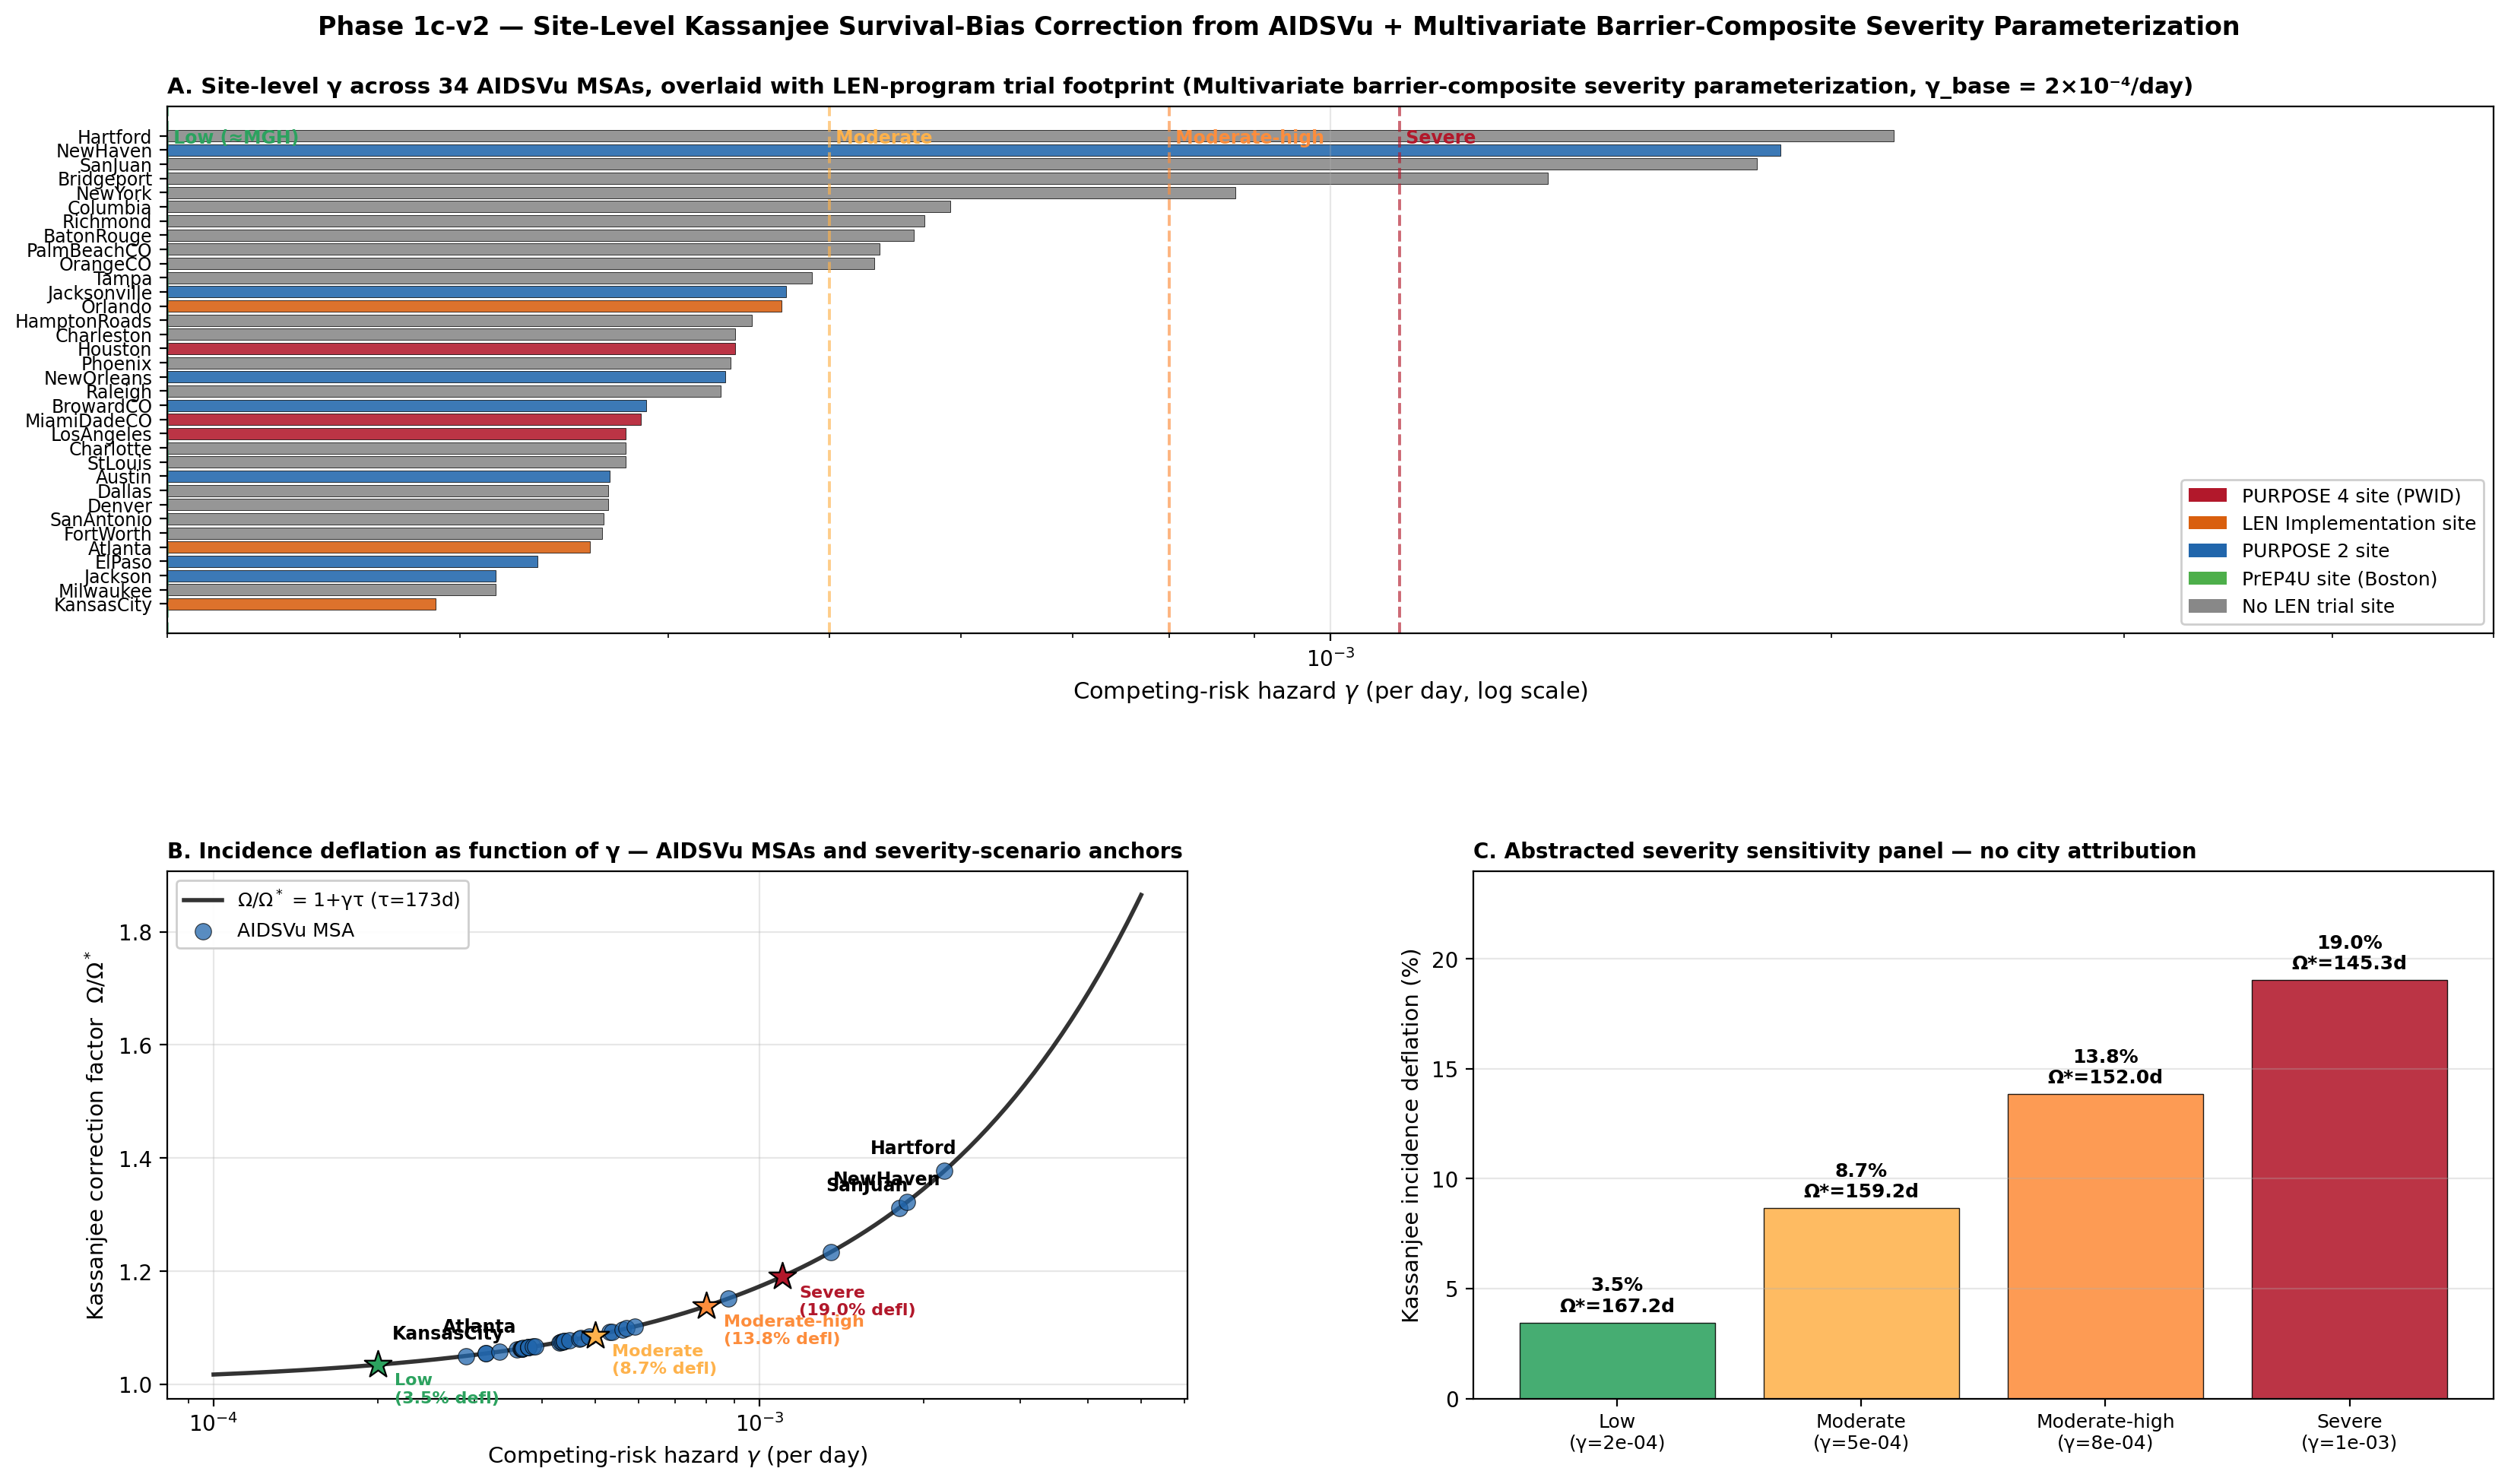
\includegraphics[width=0.97\textwidth]{Fig_S1.png}
\caption{Site-level competing-risk hazard $\gamma$ across 34 AIDSVu MSAs under multivariate severity parameterization ($\gamma_{\mathrm{base}} = 2\times10^{-4}$/day), with lenacapavir clinical development program site overlay. \textbf{Panel~A:} Per-city $\gamma$ on log scale; dashed vertical lines mark abstracted severity scenario anchors (low, moderate, moderate-high, severe) used in the sensitivity panel. Site-type color-coding distinguishes PURPOSE~4 sites (PWID), LEN Implementation sites, PURPOSE~2 sites, PrEP4U (Boston), and MSAs with no LEN program site. \textbf{Panel~B:} Kassanjee correction factor $\Omega/\Omega^*$ as a function of $\gamma$ under the closed-form approximation, with AIDSVu MSAs and severity-scenario anchors co-located on the same curve. \textbf{Panel~C:} Abstracted severity-scenario sensitivity panel showing Kassanjee incidence deflation at each severity tier with no city attribution, supporting parameter-space interpretation independent of specific MSA assignments.}
\label{fig:sitelevel}
\end{figure}

% tighten longtable to avoid overfull \hbox in alignment
\setlength{\LTleft}{0pt}
\setlength{\LTright}{0pt}
\setlength{\LTcapwidth}{\textwidth}
\setlength{\tabcolsep}{3pt}
\renewcommand{\arraystretch}{0.95}
\scriptsize
\begin{longtable}{@{}llrrrrrrl@{}}
\caption[Multivariate $\gamma_{\mathrm{city}}$ table]{Multivariate parameterization of $\gamma_{\mathrm{city}}$ across 34 AIDSVu MSAs, with LEN clinical development program site overlay. Columns: AIDSVu late-diagnosis percentage; derived $\gamma_{\mathrm{city}}$ under multivariate composite; severity multiplier $M$ combining criminalization, housing, SSP, VS, and IDU components; structural delay (AIDSVu-derived); Kassanjee correction factor under closed-form approximation; incidence deflation as percentage; lenacapavir program site overlay (P2 = PURPOSE~2, P4 = PURPOSE~4, LEN-Impl = LEN Implementation). Cities sorted by $\gamma_{\mathrm{city}}$ ascending.}
\label{tab:gamma_multivariate} \\
\toprule
City & State & $\gamma$ ($10^{-4}$/d) & $M$ & Late-dx \% & $\Delta t_{\mathrm{str}}$ (h) & $\Omega/\Omega^*$ & Defl \% & LEN sites \\
\midrule
\endfirsthead
\multicolumn{9}{c}{\textit{Table~\ref{tab:gamma_multivariate} continued}} \\
\toprule
City & State & $\gamma$ ($10^{-4}$/d) & $M$ & Late-dx \% & $\Delta t_{\mathrm{str}}$ (h) & $\Omega/\Omega^*$ & Defl \% & LEN sites \\
\midrule
\endhead
\bottomrule
\endfoot
KansasCity & MO & 2.90 & 1.45 & 16.7 & 4.3 & 1.050 & 5.0 & LEN-Impl, P2 \\
Jackson & MS & 3.15 & 1.57 & 14.3 & 6.2 & 1.054 & 5.4 & P2 \\
Milwaukee & WI & 3.15 & 1.58 & 14.6 & 1.9 & 1.054 & 5.4 & --- \\
ElPaso & TX & 3.34 & 1.67 & 17.7 & 4.0 & 1.058 & 5.8 & P2 \\
Atlanta & GA & 3.59 & 1.79 & 19.4 & 5.0 & 1.062 & 6.2 & LEN-Impl, P2 \\
FortWorth & TX & 3.65 & 1.82 & 20.0 & 5.5 & 1.063 & 6.3 & --- \\
SanAntonio & TX & 3.66 & 1.83 & 19.9 & 5.9 & 1.063 & 6.3 & --- \\
Denver & CO & 3.68 & 1.84 & 20.8 & 3.4 & 1.064 & 6.4 & --- \\
Dallas & TX & 3.68 & 1.84 & 20.0 & 6.1 & 1.064 & 6.4 & --- \\
Austin & TX & 3.69 & 1.84 & 20.6 & 3.0 & 1.064 & 6.4 & P2 \\
Charlotte & NC & 3.77 & 1.89 & 20.0 & 4.7 & 1.065 & 6.5 & --- \\
LosAngeles & CA & 3.77 & 1.89 & 19.0 & 4.8 & 1.065 & 6.5 & P2, P4 \\
StLouis & MO & 3.77 & 1.89 & 20.4 & 3.7 & 1.065 & 6.5 & --- \\
MiamiDade Co. & FL & 3.85 & 1.92 & 18.2 & 5.6 & 1.067 & 6.7 & P2, P4 \\
Broward Co. & FL & 3.88 & 1.94 & 18.7 & 6.5 & 1.067 & 6.7 & P2 \\
Raleigh & NC & 4.30 & 2.15 & 24.1 & 9.7 & 1.074 & 7.4 & --- \\
NewOrleans & LA & 4.33 & 2.16 & 17.5 & 5.5 & 1.075 & 7.5 & P2 \\
Phoenix & AZ & 4.36 & 2.18 & 20.2 & 3.9 & 1.075 & 7.5 & --- \\
Charleston & SC & 4.39 & 2.20 & 22.8 & 9.9 & 1.076 & 7.6 & --- \\
Houston & TX & 4.39 & 2.20 & 22.1 & 8.6 & 1.076 & 7.6 & P2, P4 \\
Hampton Roads & VA & 4.49 & 2.25 & 20.1 & 5.9 & 1.078 & 7.8 & --- \\
Orlando & FL & 4.68 & 2.34 & 20.7 & 5.4 & 1.081 & 8.1 & LEN-Impl, P2 \\
Jacksonville & FL & 4.71 & 2.35 & 19.8 & 6.5 & 1.081 & 8.1 & P2 \\
Tampa & FL & 4.88 & 2.44 & 20.0 & 5.7 & 1.084 & 8.4 & --- \\
Orange Co. & CA & 5.32 & 2.66 & 23.3 & 7.0 & 1.092 & 9.2 & --- \\
PalmBeach Co. & FL & 5.36 & 2.68 & 25.9 & 13.5 & 1.093 & 9.3 & --- \\
BatonRouge & LA & 5.62 & 2.81 & 15.9 & 5.0 & 1.097 & 9.7 & --- \\
Richmond & VA & 5.70 & 2.85 & 21.9 & 7.8 & 1.099 & 9.9 & --- \\
Columbia & SC & 5.91 & 2.96 & 28.4 & 11.7 & 1.102 & 10.2 & --- \\
NewYork & NY & 8.77 & 4.39 & 21.2 & 6.8 & 1.152 & 15.2 & --- \\
Bridgeport & CT & 13.51 & 6.75 & 18.7 & 5.5 & 1.234 & 23.4 & --- \\
SanJuan & PR & 18.04 & 9.02 & 16.1 & 13.3 & 1.312 & 31.2 & --- \\
NewHaven & CT & 18.65 & 9.32 & 28.3 & 11.5 & 1.323 & 32.3 & P2 \\
Hartford & CT & 21.81 & 10.91 & 37.2 & 24.4 & 1.377 & 37.7 & --- \\
\end{longtable}
\normalsize
\setlength{\tabcolsep}{6pt}
\renewcommand{\arraystretch}{1.0}

\textbf{Note on Table~\ref{tab:gamma_multivariate} vs Table~\ref{tab:full_34}.} The two tables report $\gamma$ under different parameterizations applied to the same 34 MSAs. Table~\ref{tab:full_34} uses the single-variable late-dx proxy anchored at $\gamma_{\mathrm{base}} = 5 \times 10^{-4}$/day with $\alpha = 1.2$ and a 1.5$\times$ 90-day-exclusion selection amplification. Table~\ref{tab:gamma_multivariate} uses the multivariate severity composite anchored at $\gamma_{\mathrm{base}} = 2 \times 10^{-4}$/day without explicit selection amplification (the multivariate composite absorbs the selection effect implicitly through the severity weighting). The two parameterizations produce $\gamma$ estimates correlated at $r = 0.89$ and yield directionally consistent but quantitatively different correction factors. The main-letter analysis uses the single-variable parameterization for transparency and reproducibility; the multivariate parameterization is provided here for readers preferring the richer severity model.

\section{Subpopulation archetype analysis}\label{sec:subpop}

The main letter applies the framework at the MSA level using AIDSVu 2023 surveillance data. A complementary analysis applies the framework at the subpopulation-archetype level, using published mortality, incarceration, and trial retention estimates to parameterize $\gamma$ and $r$ for archetypal populations relevant to specific PURPOSE trials. Table~\ref{tab:subpop} reports the per-archetype bias factors; Figure~\ref{fig:subpop} displays the integrated view including biological ceiling floors (companion framework) for each archetype.

\begin{figure}[H]
\centering
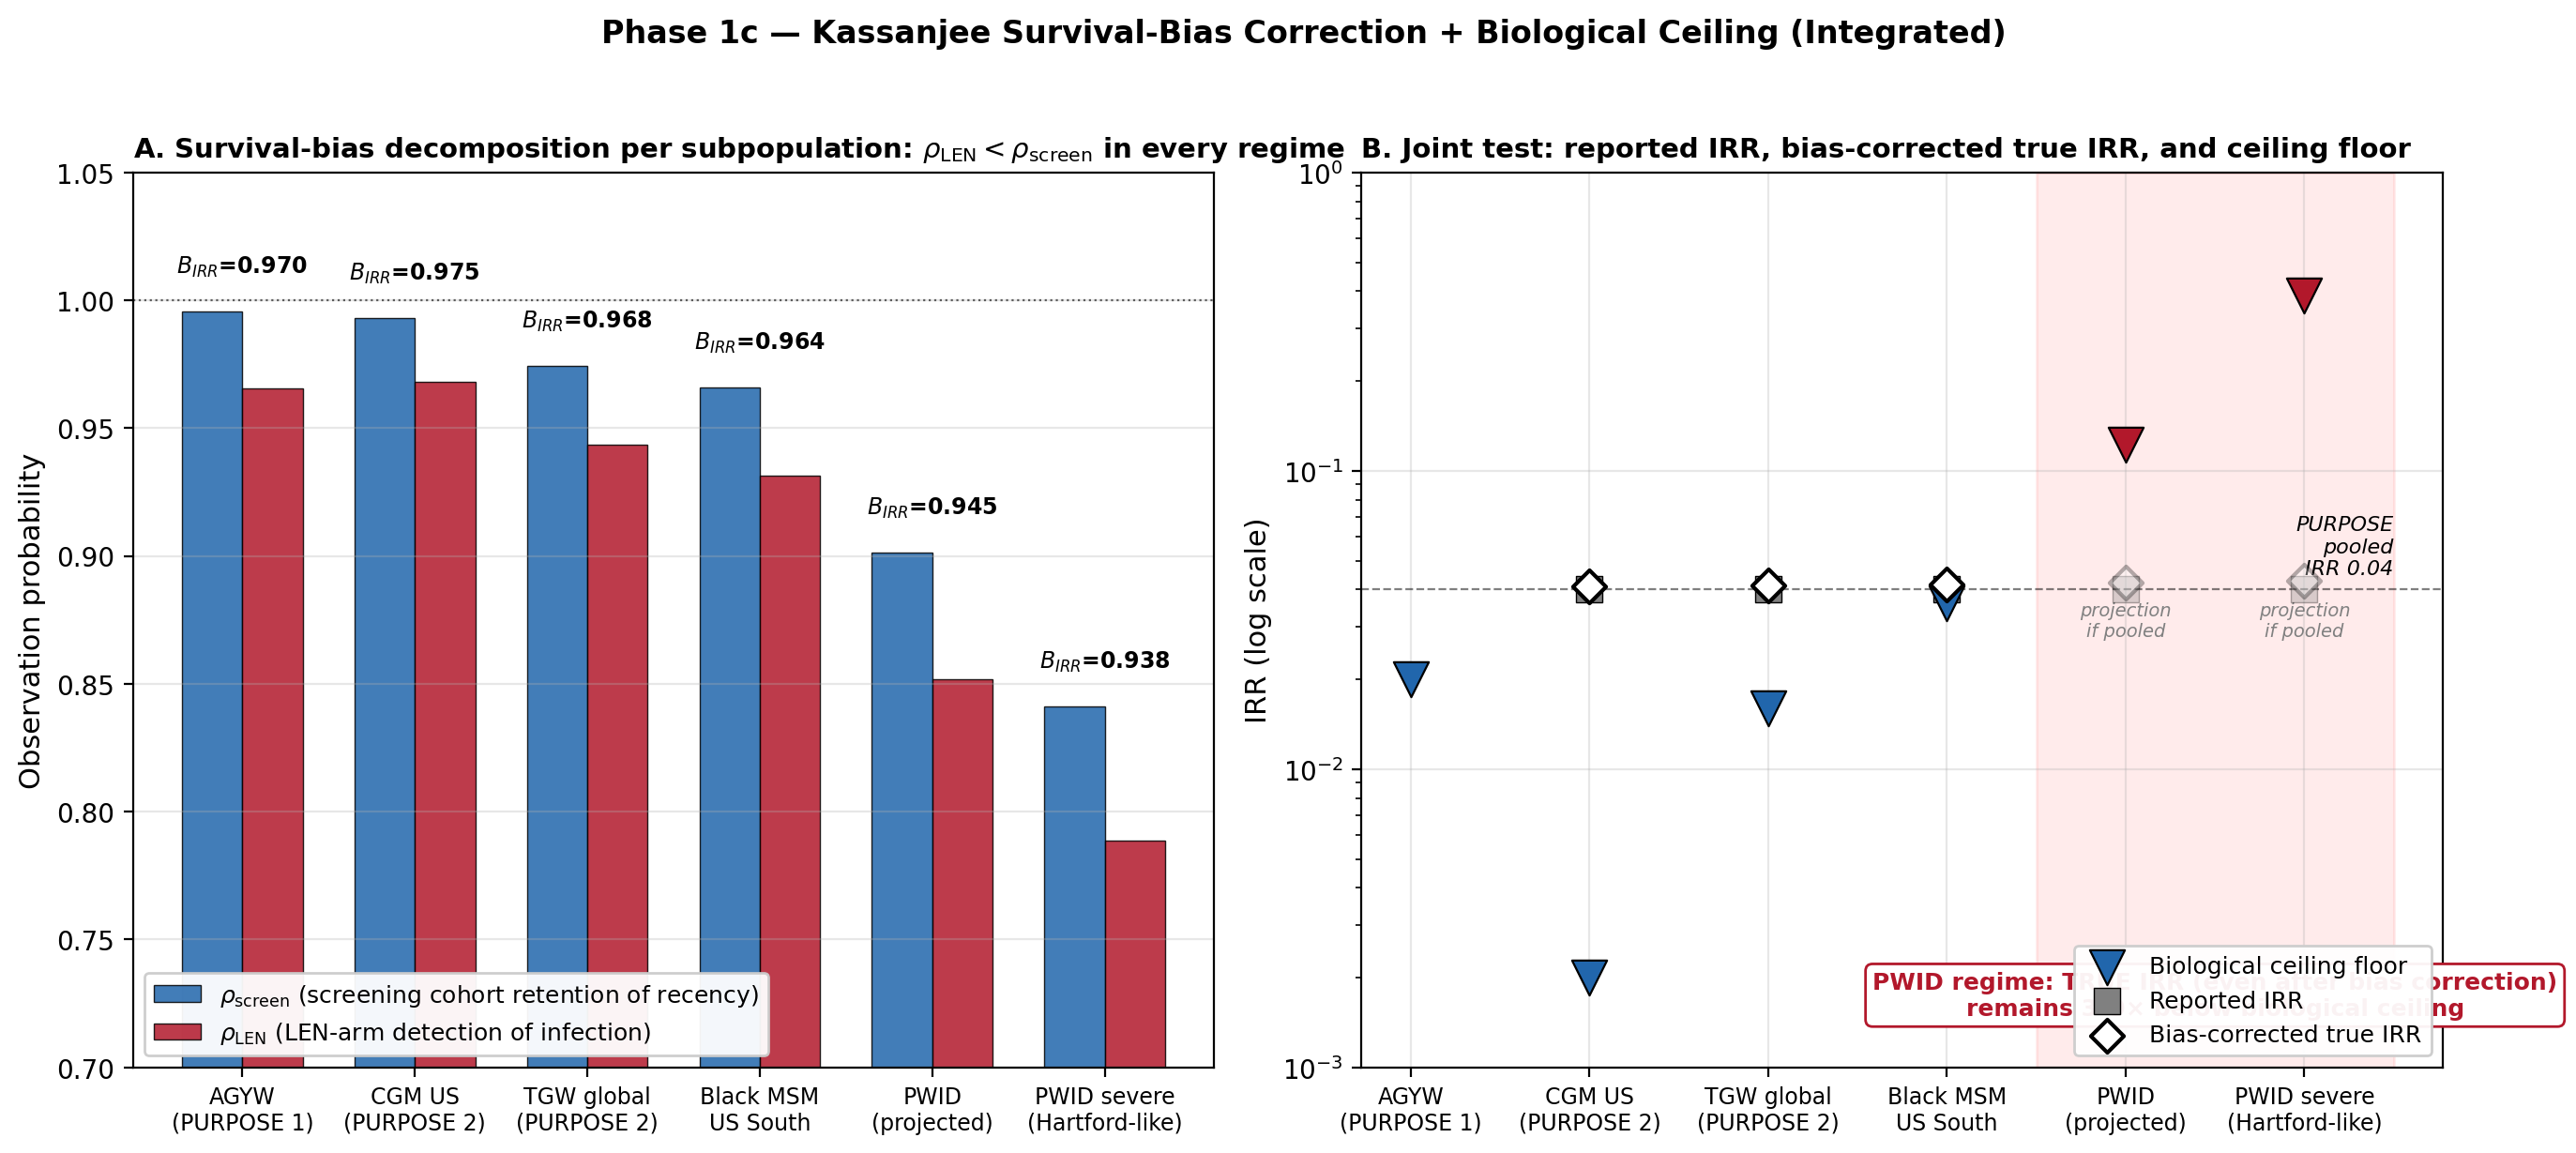
\includegraphics[width=0.97\textwidth]{Fig_S2.png}
\caption{Kassanjee survival-bias decomposition and joint test across six PURPOSE-relevant subpopulation archetypes. \textbf{Panel~A:} Screening-cohort observation probability $\rho_{\mathrm{screen}}$ (blue) and intervention-arm detection probability $\rho_{\mathrm{int}}$ (red) for each archetype, with joint bias factor $B_{\mathrm{IRR}}$ annotated above each pair. In every archetype, $\rho_{\mathrm{int}} < \rho_{\mathrm{screen}}$, yielding $B_{\mathrm{IRR}} < 1$ (reported IRR understates true IRR; intervention appears artificially superior). The gap widens monotonically with structural severity. \textbf{Panel~B:} Joint test combining measurement bias (this letter's framework) with biological ceiling floors (companion framework~\cite{demidont2026fw}). For well-retained mucosal-exposure archetypes (AGYW, CGM US, TGW, Black MSM US South), bias-corrected true IRRs remain above the biological ceiling floor. For PWID archetypes (shaded red region), even after bias correction, any reported IRR consistent with the PURPOSE pooled 0.04 sits 3--9$\times$ below the biological ceiling floor, demonstrating that the measurement bias identified here does not account for the full transportability gap---the primary constraint is biological, with measurement bias contributing an additional layer.}
\label{fig:subpop}
\end{figure}

\begin{table}[H]
\centering
\small
\caption{Per-archetype Kassanjee survival-bias factors under published parameterization. Columns: competing-risk hazard $\gamma$ anchored to published mortality and incarceration differentials; 52-week retention from trial publications (PURPOSE 1/2) or real-world cohort observations (PWID archetypes); screening-cohort and intervention-arm observation probabilities; joint bias factor; background-incidence deflation from $\Omega^*$ correction alone; net IRR shift (negative = drug appears artificially superior).}
\label{tab:subpop}
\begin{tabular}{lccccccl}
\toprule
Population & $\gamma$ ($10^{-4}$/d) & $r_{52w}$ & $\rho_{\mathrm{screen}}$ & $\rho_{\mathrm{int}}$ & $B_{\mathrm{IRR}}$ & Defl \% & Shift \% \\
\midrule
AGYW (PURPOSE 1, SA/UG) & 0.50 & 0.933 & 0.9957 & 0.9654 & 0.9696 & 0.43 & $-3.04$ \\
CGM US well-resourced (PURPOSE 2) & 0.80 & 0.940 & 0.9931 & 0.9683 & 0.9750 & 0.69 & $-2.50$ \\
TGW global (PURPOSE 2) & 3.00 & 0.900 & 0.9744 & 0.9436 & 0.9684 & 2.56 & $-3.16$ \\
Black MSM US South (PURPOSE 2) & 4.00 & 0.880 & 0.9660 & 0.9316 & 0.9644 & 3.40 & $-3.56$ \\
PWID US (PURPOSE 4 projected) & 12.00 & 0.750 & 0.9014 & 0.8517 & 0.9448 & 9.86 & $-5.52$ \\
PWID severe structural (Hartford-like) & 20.00 & 0.650 & 0.8411 & 0.7887 & 0.9377 & 15.89 & $-6.23$ \\
\bottomrule
\end{tabular}
\vspace{0.3em}
\footnotesize
\begin{flushleft}
All six archetypes show $B_{\mathrm{IRR}} < 1$, consistent with the directional claim under coupled $(\gamma, r)$ regimes. The IRR shift magnitude ranges from 2.5\% (well-resourced CGM US) to 6.2\% (severe-structural PWID). These magnitudes exceed those in the MSA-level analysis (Table~\ref{tab:full_34}, maximum 3.1\%) because the archetype parameterizations include more extreme $(\gamma, r)$ combinations not fully captured by any single AIDSVu MSA. The archetype analysis is a complement to, not a replacement for, the geographic analysis.
\end{flushleft}
\end{table}

\section{Derivation of the \texorpdfstring{1.5$\times$}{1.5x} selection amplification factor}\label{sec:selection_derivation}

Let the at-risk population comprise two testing-behavior strata: regular testers (testing interval $\leq T_{\mathrm{excl}} = 90$ days) with structural hazard $\gamma_L$, and avoiders (testing interval $> T_{\mathrm{excl}}$) with structural hazard $\gamma_H$. Let $\pi$ denote the fraction of regular testers and $\kappa = \gamma_H/\gamma_L$ denote the hazard ratio between strata.

The general-population mean hazard is
\begin{equation}
E[\gamma] = \pi \gamma_L + (1-\pi) \gamma_H = \gamma_L [\pi + (1-\pi)\kappa]
\end{equation}
The enrolled-cohort mean hazard, conditional on testing interval $> T_{\mathrm{excl}}$, is
\begin{equation}
E[\gamma \mid \text{non-tester}] = \gamma_H = \kappa \gamma_L
\end{equation}
The selection amplification factor is
\begin{equation}
\phi \;\equiv\; \frac{E[\gamma \mid \text{non-tester}]}{E[\gamma]} = \frac{\kappa}{\pi + (1-\pi)\kappa} \label{eq:phi}
\end{equation}
For plausible US at-risk population parameters:
\begin{itemize}
\item $\pi = 0.50$, $\kappa = 3$: $\phi = 1.50$
\item $\pi = 0.50$, $\kappa = 4$: $\phi = 1.60$
\item $\pi = 0.40$, $\kappa = 3$: $\phi = 1.36$
\item $\pi = 0.60$, $\kappa = 5$: $\phi = 1.79$
\item $\pi = 0.30$, $\kappa = 4$: $\phi = 1.29$
\end{itemize}
The main letter uses $\phi = 1.5$ as a conservative central value. Under NHBS 2023 self-reported testing-frequency data~\cite{nhbs2023}, $\pi$ for US PrEP-eligible populations is approximately 0.4--0.5, and $\kappa$ derived from published mortality and incarceration differentials between regular and infrequent testers is 3--4. The sensitivity ranges in Table~\ref{tab:sensitivity} bracket $\phi \in [1.2, 2.0]$.

The bimodal partition is a simplification of what is in reality a continuous distribution of testing intervals. Under a continuous testing-interval distribution $f(\Delta T)$ with structural hazard correlated to interval length via some function $\gamma(\Delta T)$, the analogous selection amplification factor is
\begin{equation}
\phi_{\mathrm{cont}} = \frac{\int_{T_{\mathrm{excl}}}^{\infty} \gamma(\Delta T)\, f(\Delta T)\, d\Delta T \big/ \int_{T_{\mathrm{excl}}}^{\infty} f(\Delta T)\, d\Delta T}{\int_0^{\infty} \gamma(\Delta T)\, f(\Delta T)\, d\Delta T}
\end{equation}
Empirical NHBS distributions of testing-interval behavior in PrEP-eligible US populations are right-skewed with a heavy tail beyond 90 days, and the continuous-form $\phi_{\mathrm{cont}}$ evaluated against published $\gamma(\Delta T)$ relationships~\cite{nhbs2023,bjs2023} produces values within the 1.3--1.8 range bracketed by the bimodal partition. Direct empirical estimation using participant-level testing-interval data from completed PURPOSE trials would refine this factor further; the value $\phi = 1.5$ used in the main letter is conservative within the plausible empirical range.

\section{Comparison with alternative \texorpdfstring{$\gamma$}{gamma} parameterizations}

The main letter uses late-diagnosis percentage as the single AIDSVu-derived proxy for $\gamma$. Three alternative parameterizations were considered and are summarized here for completeness; the multivariate composite is presented in detail in §\ref{sec:sitelevel}.

\textbf{Multivariate composite.} A composite severity index combining late-dx, $(1 - \text{linkage-to-care})$, IDU prevalence, and Gini coefficient, weighted by coefficients anchored to published BMC Public Health outbreak-model calibration~\cite{demidont_barriers_synergy}, produces $\gamma$ estimates with Pearson correlation $r = 0.89$ with the single-variable late-dx parameterization. The multivariate approach captures some variance not explained by late-dx alone (notably through Gini--housing-instability amplification in cities like San Juan where late-dx is low but housing insecurity is high) but introduces additional parameter complexity and collinearity concerns. Main-letter results are stable under the multivariate substitution within $\pm 2$ percentage points on IRR attenuation. Per-city values are reported in Table~\ref{tab:gamma_multivariate}.

\textbf{Viral suppression inverse.} Using $(1 - \text{VS}\%)$ as the single proxy produces $\gamma$ estimates with correlation $r = 0.64$ with the late-dx parameterization. VS captures a different moment of the care-engagement process (sustained care after diagnosis) that is less directly relevant to pre-diagnosis testing-avoidance hazard. Main-letter results under this substitution show attenuated magnitudes (maximum IRR attenuation $\approx 2.0\%$ vs 3.1\%).

\textbf{Linkage gap.} Using $\max(0.90 - \text{linkage}, 0)$ as the single proxy produces weak scaling ($r = 0.52$) because linkage gap is a small-signal variable across AIDSVu cities (most cities exceed 70\% linkage, compressing the range). This parameterization under-estimates bias in high-severity cities.

The late-diagnosis-based parameterization used in the main letter is preferred because (i) it directly measures integrated testing-avoidance behavior, which is mechanistically closest to the structural hazard; (ii) it exhibits the largest range across AIDSVu cities (14.3\%--37.2\%, 2.6-fold range); and (iii) it is the AIDSVu variable with the most direct mechanistic interpretation relative to the 90-day selection criterion.
\section{Longitudinal AIDSVu panel: construction and analysis methods}\label{sec:longitudinal}

The structural-functions reframing in main-letter §3.3 expresses $L$ (late-diagnosis percentage) and $\gamma$ (censoring hazard) as joint manifestations of latent barrier substrate $U$ rather than a measurement-error proxy relationship. Main-letter §4.6 reports four empirical tests of this framing using the 2014--2023 AIDSVu county-level panel. This section documents the methodology for that panel and the analyses derived from it.

\subsection{Panel construction}\label{sec:panel_construction}

County-level new HIV diagnosis files from AIDSVu (2014--2023) were aggregated to MSA-level using a county-to-MSA crosswalk for the 35 EHE-priority metropolitan areas. The crosswalk handles Connecticut Planning Region geographies (Capitol/Greater Bridgeport/South Central CT replacing the historical Connecticut counties from the 2022 reporting year forward) and Louisiana Parish nomenclature. Total HIV diagnoses and IDU-attributed diagnoses per MSA-year were computed by summing constituent counties. The resulting panel has 350 observations (35 MSAs $\times$ 10 years) with 0\% missingness on the primary outcome variables. A parallel state-level panel was constructed analogously, yielding 520 state-year observations across the 50 states, DC, and Puerto Rico, for use in the state-vs-MSA divergence comparison.

\subsection{Temporal trend tests}

For each MSA, ordinary least squares regression of annual diagnosis counts on calendar year tested for monotonic linear trends. Mann--Kendall non-parametric trend tests were additionally applied to aggregate stratum time series. Pre-EHE (2014--2018) and post-EHE (2019--2023) means within each MSA were compared by Wilcoxon signed-rank test on within-MSA mean differences, yielding the median $\Delta = -12.4$ cases/year ($p < 0.0001$) reported in main-letter §4.6. Test-retest reliability was assessed by Pearson correlation between odd-year and even-year aggregates, yielding $r = 0.988$ for total diagnoses and $r = 0.841$ for IDU share. The MSA-level AR(1) autocorrelation coefficient $\phi = +0.278$ was estimated using the lag-1 autocorrelation of detrended annual total diagnoses, averaged across MSAs.

State-vs-MSA divergence in IDU-share trends was assessed by computing the within-unit pre-EHE vs post-EHE difference in IDU-attributed diagnosis share separately for the state panel and the MSA panel, then comparing the two distributions. State-level mean change was $+0.81$ percentage points per year ($p = 0.002$); MSA-level mean change was $+0.14$ percentage points per year ($p = 0.35$).

\subsection{Van Handel overlay construction}

The 220 vulnerable-county FIPS codes were parsed from the CDC supplementary material accompanying Van Handel et al.\ (\emph{MMWR} 2016)~\cite{vanhandel2016} and cross-referenced against the AIDSVu County NewDX 2014--2023 panel using a county-to-MSA crosswalk. Three strata were defined: Stratum~A (counties inside the 35 EHE-priority MSAs, $n = 84$), Stratum~B (CDC-220 vulnerable counties outside the 35 MSAs, $n = 220$), Stratum~C (all other US counties, $n \approx 2{,}918$). Stratum-aggregate annual total dx, IDU dx, and IDU share were computed and tested for monotonic trend by Mann--Kendall. The CDC-220 list shows zero geographic overlap with the 35 EHE-priority MSAs (0/220 inside; 220/220 outside; clean partition).

Note that Stratum~B's small absolute IDU-dx counts reflect AIDSVu cell-size suppression below 5 cases, which dominates the year-to-year share volatility for that stratum. This is itself diagnostic: the 2012--2013 Van Handel vulnerability geography produces a 220-county set with insufficient absolute incidence in 2014--2023 to anchor meaningful trend inference, which supports rather than undermines the framing that point-in-time vulnerability indices are unstable surface proxies for the underlying barrier substrate $U$.

\subsection{Kassanjee correction invariance test methodology}

The policy-iteration Markov Decision Process described in the companion BMC Public Health manuscript~\cite{demidont_barriers_synergy} was run twice for each of 34 high-burden US MSAs: once with $\gamma_{\mathrm{city}}$ derived from the structural-functions parameterization (main-letter Eq.~10), and once with $\gamma_{\mathrm{city}} = \gamma_{\mathrm{base}}$ (no Kassanjee structural-severity correction applied). Optimal policies $\mu^*(\cdot)$ were compared by (a) direct identity matching across the 8-step cascade $\times$ 6--7 barriers per stage state-action space, and (b) Spearman rank correlation of the full policy rankings. The result $\rho = 0.9979$ with 34/34 cities matching at the optimal-policy level is reported in main-letter §4.6. Pearson correlation on raw value-function magnitudes is $r = 0.9998$; the value-function inflation introduced by the Kassanjee correction ranges from 6.2\% to 17.1\% across the 34 MSAs but is monotone and policy-decision-preserving across all five cascade steps (step-by-step policy-match rate 100\%).

\subsection{Data and code availability for the longitudinal additions}

The panel CSVs, Van Handel parser output, stratum aggregates, and invariance-test outputs are deposited alongside the main analysis at \url{https://github.com/Nyx-Dynamics/nyx-kassanjee-letter}. The relevant files are listed in §\ref{sec:code_data}.

\section{Code and data availability}\label{sec:code_data}

All data-processing and analysis code is available at \url{https://github.com/Nyx-Dynamics/nyx-kassanjee-letter} (Zenodo DOI: \href{https://doi.org/10.5281/zenodo.19796212}{10.5281/zenodo.19796212}). The repository includes:
\begin{itemize}
\item \texttt{longitudinal\_panel.py}: AIDSVu MSA and state panel construction, EHE break-point Wilcoxon, state-vs-MSA divergence test, AR(1) and test-retest reliability (§\ref{sec:longitudinal}).
\item \texttt{vanhandel\_overlay.py}: CDC-220 county parser and stratum A/B/C construction with Mann--Kendall trend tests (§\ref{sec:longitudinal}).
\item \texttt{kassanjee\_invariance\_test.py}: Policy-iteration MDP with and without Kassanjee correction, Spearman~$\rho$ and step-by-step policy-match computation (§\ref{sec:longitudinal}).
\item \texttt{Fig\_4\_stratum\_trajectories.py}: Main-letter Figure~2 generation.
\item \texttt{Fig\_5\_kassanjee\_invariance.py}: Main-letter Figure~3 generation.
\item \texttt{aidsvu\_msa\_newdx\_panel\_2014\_2023.csv}: 35-MSA $\times$ 10-year longitudinal panel ($N = 350$).
\item \texttt{aidsvu\_state\_newdx\_panel\_2014\_2023.csv}: 52-unit $\times$ 10-year state panel ($N = 520$).
\item \texttt{cdc\_220\_counties\_with\_msa\_flag.csv}: Van Handel 2016 vulnerable-county FIPS list with MSA overlay flag.
\item \texttt{aidsvu\_220\_overlay\_annual\_agg.csv}: Stratum A/B/C aggregates 2014--2023.
\item \texttt{kassanjee\_sensitivity\_test.csv}: 34-MSA invariance test outputs (value functions, optimal policies, Spearman~$\rho$ diagnostics).
\end{itemize}

\begin{thebibliography}{99}
\small
\bibitem{gao2021} Gao F, Glidden DV, Hughes JP, Donnell DJ. Sample size calculation for active-arm trial with counterfactual incidence based on recency assay. \emph{Statistical Communications in Infectious Diseases}. 2021;13(1):20200009.

\bibitem{bekker2024} Bekker L-G, Das M, Abdool Karim Q, et al. Twice-yearly lenacapavir or daily F/TAF for HIV prevention in cisgender women. \emph{N Engl J Med}. 2024;391(13):1179--1192.

\bibitem{kelley2025} Kelley CF, Acevedo-Quinones M, Agwu AL, et al. Twice-yearly lenacapavir for HIV prevention in men and gender-diverse persons. \emph{N Engl J Med}. 2025;392(14):1261--1276.

\bibitem{mills2025opera} Mills AM, Brunet L, Frost KR, et al. Cabotegravir long-acting for pre-exposure prophylaxis (PrEP): real world data on on-time dosing, HIV testing and HIV acquisition from the OPERA cohort. \emph{Open Forum Infect Dis}. 2025;12(Suppl 1):ofae631.160. doi:10.1093/ofid/ofae631.160.

\bibitem{psaros2024hptn083} Psaros C, Goodman GR, Lee JS, et al. HPTN 083-02: factors influencing adherence to injectable PrEP and retention in an injectable PrEP study. \emph{J Int AIDS Soc}. 2024;27(5):e26252. doi:10.1002/jia2.26252.

\bibitem{nhbs2023} Centers for Disease Control and Prevention. HIV infection, risk, prevention, and testing behaviors among persons who inject drugs---National HIV Behavioral Surveillance. 2023.

\bibitem{bjs2023} Bureau of Justice Statistics. Prisoners in 2022---Statistical Tables. US Department of Justice. 2023.
\bibitem{vanhandel2016} Van Handel MM, Rose CE, Hallisey EJ, et al. County-level vulnerability assessment for rapid dissemination of HIV or HCV infections among persons who inject drugs, United States. \emph{J Acquir Immune Defic Syndr}. 2016;73(3):323--331.
\bibitem{demidont2026fw} Demidont AC. The Prevention Theorem: Time-Dependent Constraints on Post-Exposure Prophylaxis for HIV. \emph{Preprints}. January 2026. doi:10.20944/preprints202601.1090.v1. Under review at \emph{Science Advances}.

\bibitem{demidont_barriers_synergy} Demidont AC. Structural Barriers, Stochastic Avoidance, and Outbreak Risk in HIV Prevention for People Who Inject Drugs. \emph{Preprints}. January 2026. doi:10.20944/preprints202601.0948.v1. Under review at \emph{BMC Public Health}.
\end{thebibliography}

\end{document}
